%\tableofcontents
%\listoffigures
\newpage

	Alan Turing fue un matemático considerado como un precursor de la informática moderna, el diseñó la llamada máquina de Turing, esta se puede visualizar como un cabezal de lectura escritura y una banda infinita separada en secciones donde cada sección tiene cierto valor capaz de ser leído y modificado por el cabezal y a partir de este código se ejecutan acciones. \\Para ilustrarlo con un ejemplo podemos construir una máquina de Turing muy simple que lea dos símbolos \textbf{A} y \textbf{B}, A significa por ejemplo que se mueva a la derecha y B que escriba una A en lugar de la B y que se mueva a la derecha con esto fácilmente podemos modificar la cadena de  caracteres \textbf{ABABA} a \textbf{AAAAA} ya que inicia leyendo una A se mueve a la derecha lee una B, la cambia por una A y se mueve a la derecha y siguiendo este proceso llega al final de la cinta. \\En el ejemplo anterior es fácil notar que si se empieza a leer  en un lugar distinto del primer carácter es muy probable que la cadena no sea cambiada en su totalidad y estas eventualidades una maquina de Turing(MT) bien diseñada debe ser capaz de soportar. \\ Por lo general podemos realizar un diagrama de una maquina de Turing como se muestra en la Figura 1, en este diagrama podemos ver como una maquina de Turing se encarga de verificar si una cadena de números tiene una cantidad par o impar de números uno.
\begin{figure}[H]
	\centering
	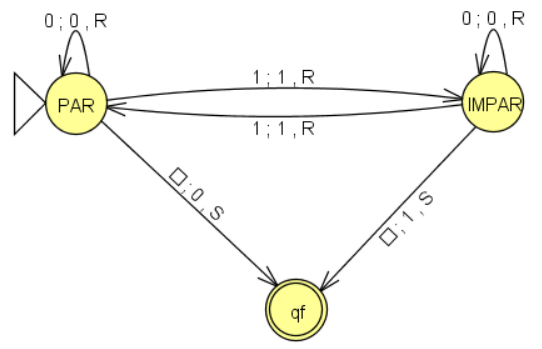
\includegraphics[width=0.5\textwidth]{./images/MAQTUR.png}
	\caption{MT que determina si una cadena tiene una cantidad de números par o impar}
\end{figure}
	
	Despues de comprender que es una MT podemos entender que es una máquina universla de Turing, esta nace gracias a las investigaciones de Alan Turing en computación y se puede definir como una MT capaz de realizar los mismos procesos de otras MT, es decir capaz de realizar muchos trabajos sin la necesidad de tener muchas máquinas, en palabras de Ramirez \textit{''recibe como entrada una máquina de Turing M y una secuencia de datos iniciales a; entonces realiza la ejecución de la maquina M con la secuencia a''}\cite{ComoMaquina} es decir es una máquina capaz de realizar cualquier proceso siempre y cuando se le envíe las instrucciones y la cinta con la que se debe trabajar como parámetro.\\Este concepto es muy importante ya que nuestras computadoras modernas parten de este principio para funcionar, es casi ilógico imaginar tener una computadora para sumar, otra para restar, otra para mostrar los resultados en pantalla, etc.\\ Básicamente nuestras computadoras son maquinas universales ya que la unidad de procesamiento es capaz de realizar múltiples acciones a la vez, gracias a que recibe instrucciones en código binario y estas instrucciones las interpreta para obtener algún resultado.
	
Gracias a Turing, a su genialidad matemática y a sus investigaciones en el campo de la computación podemos actualmente diseñar algoritmos capaces de resolver algún problema, siendo estos formulados como una MT particular, y sin sus aportes es muy difícil imaginar si la informática moderna contaría con los avances actuales siendo esta una herramienta fundamental en el desarrollo tecnológico con el que contamos actualmente.
